\documentclass[nobib,fleqn,8pt]{article}

%\\geometry{showframe}% for debugging purposes -- displays the margins

\newcommand{\bra}[1]{\left(#1\right)}
\usepackage{hyperref}
\usepackage[activate={true,nocompatibility},final,tracking=true,kerning=true,spacing=true,factor=1100,stretch=10,shrink=10]{microtype}
\usepackage{color}

% Fixes captions and images being cut off
\usepackage{marginfix}
\usepackage{mdframed}
\usepackage{xcolor}
\usepackage{pgfplots}
\usepackage[americancurrents, americaninductors, americanvoltages, americanresistors]{circuitikz}
\usepackage{siunitx}
\usepackage{amsmath,amsthm}
\usepackage{circuitikz}
\usetikzlibrary{shapes}
\usetikzlibrary{positioning}
\usetikzlibrary{arrows}

% Set up the images/graphics package
\usepackage{graphicx}
\setkeys{Gin}{width=\linewidth,totalheight=\textheight,keepaspectratio}
\graphicspath{{.}}


\newmdenv[
    backgroundcolor=black!10, % Light blue shading inside the box
    linecolor=black,         % Border color
    linewidth=1pt,          % Border thickness
    roundcorner=5pt,        % Rounded corners
    skipabove=10pt,         % Space above the box
    skipbelow=10pt,         % Space below the box
    innertopmargin=5pt,     % Inner top margin
    innerbottommargin=5pt,  % Inner bottom margin
    innerleftmargin=10pt,   % Inner left margin
    innerrightmargin=10pt   % Inner right margin
]{defbox}

\title{Notes for ECE 45600 - Integrated Circuit Design}

\date{\today}  % if the \date{} command is left out, the current date will be used

% The following package makes prettier tables.  We're all about the bling!
\usepackage{booktabs}

% The fancyvrb package lets us customize the formatting of verbatim
% environments.  We use a slightly smaller font.
\usepackage{fancyvrb}
\fvset{fontsize=\normalsize}

% Small sections of multiple columns
\usepackage{multicol}

% These commands are used to pretty-print LaTeX commands
\newcommand{\doccmd}[1]{\texttt{\textbackslash#1}}% command name -- adds backslash automatically
\newcommand{\docopt}[1]{\ensuremath{\langle}\textrm{\textit{#1}}\ensuremath{\rangle}}% optional command argument
\newcommand{\docarg}[1]{\textrm{\textit{#1}}}% (required) command argument
\newenvironment{docspec}{\begin{quote}\noindent}{\end{quote}}% command specification environment
\newcommand{\docenv}[1]{\textsf{#1}}% environment name
\newcommand{\docpkg}[1]{\texttt{#1}}% package name
\newcommand{\doccls}[1]{\texttt{#1}}% document class name
\newcommand{\docclsopt}[1]{\texttt{#1}}% document class option name

% Define a custom command for definitions
\newcommand{\defn}[2]{\noindent\textbf{#1}:\ #2}

\begin{document}

\maketitle

\begin{abstract}
    These are lecture notes for Fall 2025 ECE 45600 by professor Saeed Mohammadi at Purdue. Modify, use, and distribute as you please.
\end{abstract}

\tableofcontents

\newpage
\section{Introduction}
\subsection{Noise and Reliability}
Noise in circuits comes from undesired coupling, both capacitive and
inductive.\\
\begin{mdframed}
    Note: Capacitive and inductive coupling are reduced by:
    \begin{itemize}
        \item Placing interconnected lines far from each other.
        \item Adding ground plane between lines.
        \item Reducing length of interconnected lines
    \end{itemize}
\end{mdframed}
The following is the graph of the voltage transfer characteristics of an inverter:
\begin{center}
    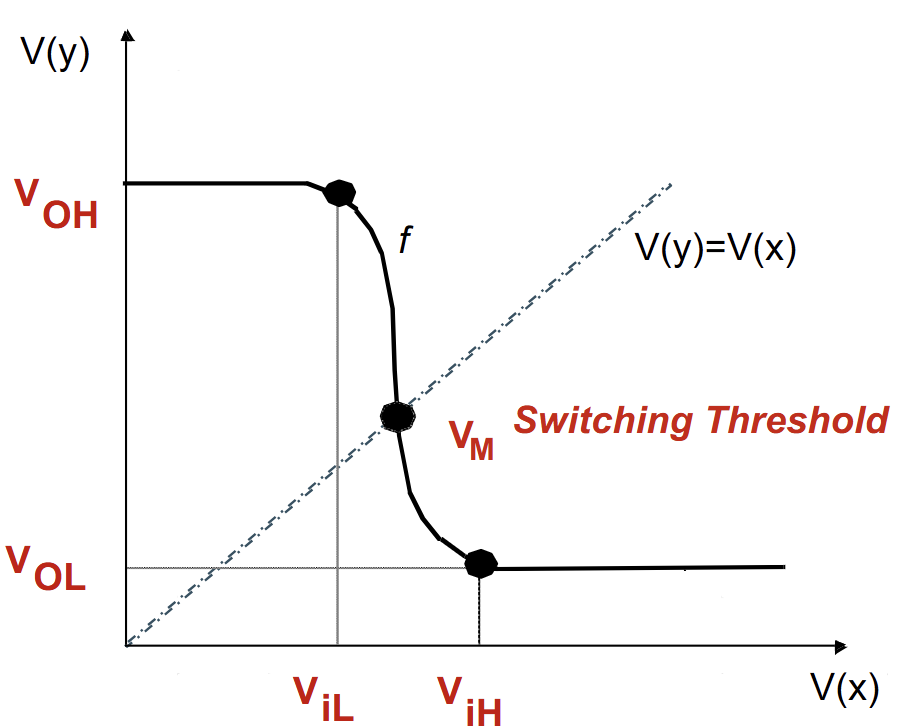
\includegraphics[width = 175px]{images/voltage_transfer_characteristics.png}
\end{center}
In it, $V_{OH} = f(V_{iH})$ is the voltage recognized as the output voltage when the inverter begins to output high. Similarly, $V_{OL} = f(V_{iL})$ is the voltage when it begins to output low. Finally, $V_M = f(V_M)$ is the point that the input and the output are the same, and is also known as the switching threshold.\\
Both $V_{iL}$ and $V_{iH}$ are points at which the curve has a slope of $-1$. The area between these two points is the undefined region, and is the reason why noise is a problem.\\
The range between the output and the input on each side of the curve is known as the noise margin, and is an area where the output is well defined into one of its two possible values:
\begin{center}
    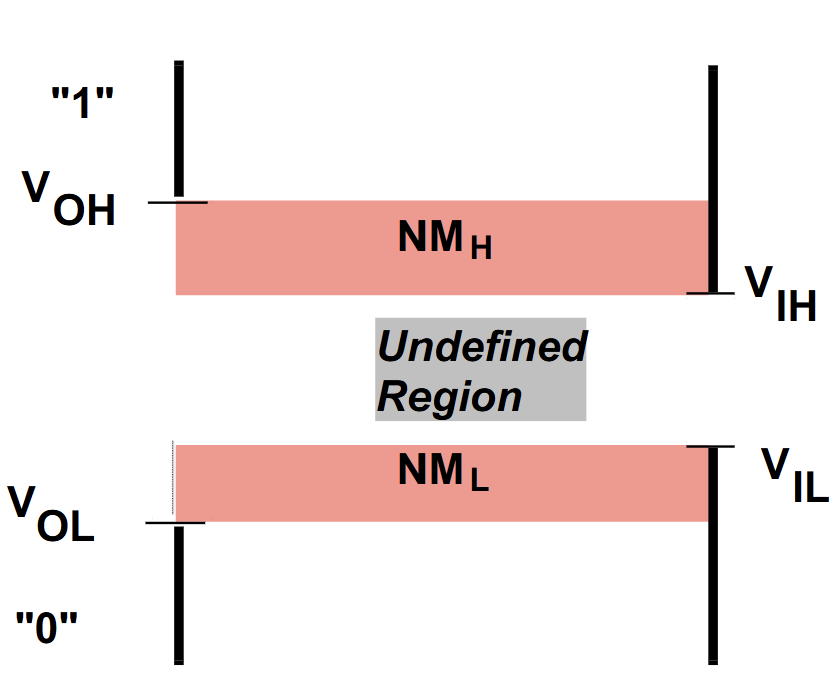
\includegraphics[width = 150px]{images/noise_margin.png}
\end{center}
There are two kinds of noise sources:
\begin{enumerate}
    \item Fixed Sources
    \item Proportional Sources
\end{enumerate}
The noise margin, $V_{NM}$, has the following properties:
\begin{equation*}
    \frac{V_{SW}}{2} \geq V_{NM}\geq \sum f_i V_{Nfi}+ \sum g_j V_{SW}
\end{equation*}
where $V_Nfi$ is a fixed noise source and $V_{SW}$ is a proportional one.\\
Noise margins are deceptive, as these can be easily disturbed, which is why the more reliable parameter is noise immunity, or the ability to suppress noise.
\begin{center}
    \includegraphics*[width = 200px]{images/noise_immunity.png}
\end{center}
The higher the impedance of the noise immunity, the more noise is rejected.\\
\subsection{Regenarative vs Non-Regenarative}
The following is a graph of a regenerative curve:
\begin{center}
    \includegraphics*[width = 150px]{images/regenerative_curve.png}
\end{center}
The behavior of this kind of curve is the following:\\
\textit{Let us imagine several inverters connected to each other in series. If the input voltage of the first inverter starts somewhere close to the center of the undefined region, after a few inverters, the output will be well into the noise margins.}\\
On the other hand, a non-regenerative curve,
\begin{center}
    \includegraphics*[width = 150px]{images/non_regenerative_curve.png}
\end{center}
\textit{In a series arrangement of inverters, if the input of one is undefined, the eventual inputs and outputs will tend to the center of the undefined region instead.}\\
This is why a regenerative curve is what we desire form our inverters.\\
\subsection{Fan-in and Fan-out}
We will now define two important terms in the context of gates: \newpage
\begin{defbox}
    The fan-in is the number of inputs a gate has, and is represented by the letter $M$:
    \begin{center}
        \includegraphics*[height = 75px]{images/fanin.png}
    \end{center}
\end{defbox}
\begin{defbox}
    The fan-out is the number of outputs a gate has, and is represented by the letter $N$:
    \begin{center}
        \includegraphics*[height = 75px]{images/fanout.png}
    \end{center}
\end{defbox}
\subsection{Gate Delays}
Another important gate parameter is the delay it possesses. The delay of a gate
will define how fast the circuit can run, as well as some restraints it will
have to avoid errors.\\ This delay, as well as its subcomponents can be seen in
the following figure:
\begin{center}
    \includegraphics*[width = 200px]{images/inverter_delay_plot.png}
\end{center}
In this image, we can see a few kinds of delays:
\begin{itemize}
    \item Fall delay $t_f$: the time it takes for the output curve to go from $V_{OH}$ to
          $V_{OL}$. Depends on the strength of the driver and the load presented to it.
    \item Fall delay $t_r$: the time it takes for the output curve to go from $V_{OL}$ to
          $V_{OH}$. Depends on the strength of the driver and the load presented to it.
    \item High to Low Propagation delay $t_{pHL}$: the time between the 50\% of the input
          to the 50\% voltage of the output when the inverter output is transitioning
          from high to low.
    \item Low to High Propagation delay $t_{pLH}$: the time between the 50\% of the input
          to the 50\% voltage of the output when the inverter output is transitioning
          from low to high.
    \item Propagation delay $t_p$: $(t_{pLH}+t_{pHL})/2$
\end{itemize}
Now, let us imagine the following circuit:
\begin{center}
    \includegraphics*[width = 200px]{images/inverter_cycle.png}
\end{center}
The input of the first inverter will be bouncing between high and low at a certain frequency, and thus we can deduce the propagation delay using the following formula:
\begin{equation*}
    T = 2 \times t_p \times N
\end{equation*}
\subsection{Inverter Modelling}
We can use an RC circuit to model the delay of an inverter as shown below:
\begin{center}
    \includegraphics*[width = 120px]{images/rc_inverter_delay.png}
\end{center}
This will work if the following two properties, brought about by their definitions withing the delay curve and the voltage transfer characteristics curve, hold true:
\begin{eqnarray*}
    t_p = \ln(2)\tau\\
    t_r \approx t_f = \ln(9)\tau
\end{eqnarray*}
\subsubsection{Power Dissipation}
We know the following definitions of power:
\begin{itemize}
    \item Instantaneous: $p(t) = v(t)i(t) = V_{supply} i(t)$
    \item Peak: $P_{peak} = V_{supply}i_{peak}$
    \item Average: $P_{ave} = \frac{1}{T}\int_{t}^{t+T}p(t)dt =
              \frac{V_{supply}}{T}\int_{t}^{t+T} i_{supply}(t)dt$
\end{itemize}
which lead to the following energy definitions:
\begin{itemize}
    \item Power-Delay Product (PDP): $E = \text{Energy per operation} = P_{ave}\times t$
    \item Energy-Delayed Product (EDP): $\text{quality metric of gate} = E \times t_p$
\end{itemize}
The energy consumption due to transitions (there is no power dissipated when there is no transition) is the following:
\begin{eqnarray}
    E_{0\rightarrow 1} = C_L * V_{dd}^2\\
    E_{cap} = \frac{1}{2}C_L * V_{dd}^2
\end{eqnarray}
As can be seen in equation (2), half the energy is stored in the capacitor. That is, half the energy is dissipated into the atmosphere by the resistor.\\
\section{CMOS Technology}
The following is the structure of a modern NMOS transistor:
\begin{center}
    \includegraphics*[height = 125px]{images/modern_cmos_composition.png}
\end{center}
\begin{mdframed}
    \textbf{Note}: The process described is over 20 years old now.    
\end{mdframed}
The silicon substrate ($p^+$) is about $400\mu m - 500\mu m$ thick. \\
Above it we have another layer of a more clean silicon substrate (p-epi) that is placed by introducing wafers to vacuum chambers with silicon gas, allowing the silicon to be deposited appropriately. The (p-epi) layer only needs to be $0.1\mu m$ thick, but the optimal range that avoids the most imperfections is between $1\mu m-2\mu m$.\\
The next layer to be placed is a layer of $SiO_2$, which is created by heating the water to $1050^\circ C$ and allowing the molecules of oxygen to bond with the silicon. This layer is about 200Ang (20nm) thick.\\
Next, the polymer is spread across the whole wafer. This is done by placing a small amount of the liquid polymer, before rotating it at high speeds and allowing the polymer to spread approximately evenly across the wafer. The thickness depends on the viscosity of the polymer as well as the rotation speed.\\
Based on the thickness of the polymer, the duration of the hardening exposure in the lithography is determined. The photomask is defined by covering the areas that do not want to be kept (using laser etched glass), and thus are not hardened when exposing the wafer to the UV light. The soft part is then dissolved and removed.\\
The trenches left from removing the undesired parts are filled with oxide, this time, it is not a high quality oxide like in the previous $SiO_2$ layer. This leaves an uneven layer, which is planarized using chemical-mechanical polishing (CMP). \\
Another mask is placed on the wafer. Ions from elements from group 5 like Phosphorus (Ph), Arsenic (As) or Nitrogen (N) are accelerated through a few kV and blasted at the layer over the non-trench parts. The ions harmlessly cross the oxide layer and allow the n-doped region to be doped. This layer has about $10^{16} ions/cm^3$, as opposed to the approximately $10^{23} atoms/cm^3$ of silicon.\\
The same is done to create the p-doped region, but with elements from group 3 like Boron (B), Aluminum (Al) or Gallium (Ga).\\
The wafer is then heated to about $900^\circ C$ to allow the ions to bond with the silicon. From this point onward, temperatures above around $800^\circ C$ are unacceptable, as they will diffuse the doping.\\
Thus, Low-Pressure Chemical Vapor Deposition (LPCVD) is used to deposit a poly-silicon. A 100nm thick, 45nm wide undoped material is deposited. 3 regions, one on the poly of one side and the other two around the poly of the other side are created, and within them the desired material (group 5 for NMOS, group 3 for PMOS) is implanted. The opposite is then done, the windows are replaced, and so is the element. This leaves wither poly doped with p, directly surrounded by p and then surrounded by n, or doped with n surrounded by p.\\
The polysilicon will be the gate, directly surrounded by source and drain, and externally surrounded by the body.

\begin{mdframed}
    \textbf{Note}: The substrate is created by melting sand at about $1500^\circ C$, allowing the gas bubbles within to escape. After this, they place a seed of silicon within the fluid. They then extract the seed, while rotating the molten silicon very slowly. This allows the silicon to crystallize in a structure based on the seed. The resulting crystal is several meters tall, and a few inches in radius. The result is finally cut into approximately half a mm thick slices called wafers.
\end{mdframed}
The following is an image of the lithographical representation of two NMOS (below) and two PMOS (above) transistors connected:
\begin{center}
    \includegraphics*[width = 125px]{images/pmos_nmos_lithography.png}
\end{center}
The overlap between purple and green is the area where the transistors are.
\begin{mdframed}
    The PMOS transistors are notably larger, as they are slower, and the size compensates for this.
\end{mdframed}

\subsection{Design Rules and Limitations}
When making transistors, certain design rules must be followed. These are predefined, and help avoid production flaws. The software, Cadence in this case, checks for the fulfillment of these rules.\\
There are two kinds of design rules:
\begin{enumerate}
    \item Scalable: lambda parameter which represents half the minimum length. They allow for rules to pass from one process to another.
    \item Absolute: applicable to more specific situations.
\end{enumerate}
When designing an IC, the software tries to automatically generate a layout that fulfills all its rules. The user can modify the layouts, but they might violate some of these rules.\\
After the chip is designed, it is sent to be fabricated and packaged. Then the IC can be placed on a PCB.\\

\end{document}
